\section{Uitvoering en resultaten}
% In dit hoofdstuk wordt de daadwerkelijke uitvoering van de practice based research beschreven, waarbij de in het hoofdstuk methode beschreven aanpak wordt gevolgd. De verhouding tussen praktijk in de vorm van projecten en onderbouwing kan flink uiteenlopen, van 80/20% tot 20/80%. De thesis is daarbij niet alleen een droog projectverslag. De nadruk moet op de verantwoording liggen: reflectie op de relatie tussen de gevolgde aanpak aanpak en resultaten.

\subsection{Onderbouwen aannames}

In dit hoofdstuk ga ik de gemaakte aannames verder beschrijven en beargumenteren.

\subsubsection*{Vernieuwd luistergedrag}

\begin{quotebox}
Door het vernieuwde luistergedrag binnen streamingdiensten heeft het album als distributievorm zijn individuele waarde verloren.
\end{quotebox}

Streamingdiensten zoals Spotify hebben het luistergedrag van mensen merkbaar veranderd. Waar in de tijd van de LP en CD veel werd geluisterd naar albums is deze vorm van publiceren van muziek steeds minder vanzelfsprekend. Hoewel albums nog steeds worden gebruikt, wordt de muziek nu vaak ook tussendoor gepubliceerd als losse nummers (singles), of in de vorm van een EP met 3 a 4 nummers.

Dit heeft meerdere oorzaken: de eerste is dat het via streamingdiensten makkelijker is om losse releases te doen. Er is geen fysiek medium wat gedrukt en geleverd moet worden, maar een online dienst waarbij de content overal tegelijk beschikbaar is. Artiesten hoeven daarom niet meer te wachten tot ze genoeg nummers hebben voor een album, maar kunnen direct een nummer uitbrengen. Het is voor de artiest makkelijker om een los nummer te maken dan een heel album. Een album moet een geheel zijn, waarbij de nummers op elkaar aansluiten. Vaak heeft een album een overkoepelend thema, of verteld het een doorlopend verhaal (concept album). Een album heeft hierdoor automatisch meer waarde dan het losse nummer omdat het een complexer en groter geheel is.

Een andere reden is dat de manier waarom mensen muziek vinden is veranderd. Er wordt nu veel meer geluisterd via playlists. Binnen deze playlists is muziek van meerdere artiesten  binnen eenzelfde genre gebundeld. De luisteraar hoeft niet meer zelf op zoek naar nieuwe muziek, maar kan dit overlaten aan de curator en het algoritme van de playlist.

Door de focus op losse nummers en playlists kan de context van een album verloren gaan. Artiesten moeten nu nadenken over hoe ze hun muziek het beste kunnen presenteren in een wereld waarin singles de norm zijn geworden. Het album verandert hiermee van standaard distributiemedium naar meer conceptuele vorm. Dit heeft ook gevolgen voor de manier waarop de muziek gepromoot wordt.

Deze verandering in luistergedrag hoeft niet direct gezien te worden als een probleem. Het is echter wel belangrijk om te beseffen dat deze verschuiving plaats vindt en dat het invloed kan hebben op verschillende aspecten van de muziekindustrie, van de manier waarop artiesten muziek maken en presenteren tot de marketingstrategieën en het succes van artiesten.

\subsubsection*{Waarde verschoven naar platform}
\todo{Braindump en AI}
\begin{quotebox}
De waarde zit op dit moment niet meer in de muziek, maar in het platform dat toegang biedt tot de voor de luisteraar haast onbeperkte hoeveelheid aan content.
\end{quotebox}

Voor luisteraars is de waarde nu voornamelijk te vinden in het platform waar de muziek te luisteren is. Dit komt door de grote hoeveelheid muziek, die vrijwel direct af te spelen is op het eigen apparaat.

Luisteraars betalen niet meer voor de muziek, maar voor de toegang tot het platform. De waarde van het platform zit in de gebruiksvriendelijkheid, de aanbevelingen, de mogelijkheid om playlists te maken en te delen, en de grote database aan content die streamingdiensten bieden. Deze platforms stellen luisteraars in staat om nieuwe muziek te ontdekken zonder dat ze hiervoor naar een fysieke winkel moeten gaan.

Een nieuw probleem is dat de betaling van artiesten een groot grijs gebied is. Gebruikers van streamingdiensten betalen een vast bedrag per maand, wat vervolgens wordt verdeeld over de artiesten. Hoe dit precies gebeurt heeft de luisteraar vrijwel geen inzicht in. De luisteraar betaald voor de toegang tot het platform, en niet voor de muziek, wat vervolgens ervoor zorgt dat de luisteraar minder waarde hecht aan de muziek zelf, maar meer aan het platform.

\subsubsection*{Waarde zit in community}
\todo{Braindump en AI}
\begin{quotebox}
De waarde van muziek zit in de community die wordt gevormd rondom de muziek.
\end{quotebox}

Muziek wordt al duizenden jaren gebruikt door mensen om zich te identificeren binnen een cultuur.

Artiesten zijn, mede door tegenvallende inkomsten uit streaming diensten, meer aan het focussen op het bouwen van hun community. Dit doen ze vaak via sociale media kanalen waar ze direct contact kunnen hebben met hun fans. Zo delen ze persoonlijke video's, backstage beelden en andere content die niet direct met de muziek te maken heeft. Dit zorgt ervoor dat de fans zich meer verbonden voelen met de artiest, en daardoor meer geneigd zijn om de muziek te kopen.

In de jaren 80 was binnen de popmuziek een erg gesegmenteerde cultuur. Platenmaatschappijen forceerden sterk een wij-tegen-zij mentaliteit, met als gevolg dat fans van verschillende artiesten tegenover elkaar kwamen te staan. De reden hierachter was om meer publiciteit te genereren voor de artiesten. Door de fans tegen elkaar op te zetten zouden ze meer muziek kopen om hun eigen artiest te steunen. Tegenwoordig is dit heel anders. Hoewel er nog steeds 'echte fans' van artiesten zijn, identificeert men zich nu meer  met genres.

Genres als Metal en KPop bouwen sterk op een hechte fanbase per artiest. Merchandise is hierbij erg belangrijk, omdat daarmee wordt laten zien dat je bij de community hoort. Het hebben van merch, en het kunnen zeggen dat je naar een bepaald optreden bent geweest, is soms net zo belangrijk als de muziek zelf.

\subsubsection*{Beginnende artiesten niet rendabel}
\todo{Braindump en AI}
\begin{quotebox}
Doordat beginnende artiesten op streamingdiensten direct concurreren met artiesten op professioneel niveau is het moeilijk om door te breken. Dit is slecht voor de diversiteit en innovatie binnen de muziekindustrie.
\end{quotebox}

\begin{comment}
Doordat beginnende artiesten niet rendabel zijn is het een grote drempel om volledig (financieel) te focussen op muziek. Hierdoor stoppen veel beginnende artiesten met muziek maken, of brengen ze minder muziek uit.
\end{comment}

Het netwerkeffect van streamingdiensten zorgt er voor dat het grootste deel van de inkomsten bij de grote artiesten terecht komt, zeker in vergelijking met de traditionele muziekindustrie.
Doordat beginnende artiesten niet rendabel zijn is het een grote drempel om volledig (financieel) te focussen op muziek. Hierdoor stoppen veel beginnende artiesten met muziek maken, of brengen ze minder muziek uit. Dit is een kwalitatief probleem.

\begin{comment}
  CHATGPT OUTPUT:

  Het gebrek aan mogelijkheden voor beginnende artiesten om door te breken op streamingdiensten heeft negatieve gevolgen voor de diversiteit en innovatie binnen de muziekindustrie. Wanneer beginnende artiesten direct concurreren met gevestigde professionals, worden ze vaak over het hoofd gezien vanwege de populariteit en zichtbaarheid van de bekendere artiesten.

  Het netwerkeffect van streamingdiensten versterkt dit probleem doordat de meeste inkomsten naar de grote artiesten gaan, vooral in vergelijking met de traditionele muziekindustrie. Dit betekent dat beginnende artiesten vaak niet rendabel zijn en het moeilijk hebben om financieel te kunnen focussen op hun muziekcarrière. Het gebrek aan financiële ondersteuning vormt een grote drempel voor hen, waardoor ze gedwongen worden om hun muzikale ambities op te geven of minder muziek uit te brengen.

  Dit kwalitatieve probleem heeft gevolgen voor de muziekwereld als geheel. Beginnende artiesten brengen vaak nieuwe ideeën, frisse perspectieven en innovatieve geluiden met zich mee. Ze zorgen voor diversiteit in genres, stijlen en creatieve benaderingen. Wanneer deze opkomende talenten worden ontmoedigd of beperkt in hun mogelijkheden om zich te uiten, leidt dit tot een gebrek aan vernieuwing en variatie in de muziek die beschikbaar is voor het publiek.

  Bovendien is de diversiteit binnen de muziekindustrie van cruciaal belang voor het creëren van een inclusieve samenleving. Muziek weerspiegelt de verschillende culturen, achtergronden en ervaringen van mensen over de hele wereld. Door beginnende artiesten de kans te geven om gehoord te worden, kunnen nieuwe stemmen opkomen en krijgen minder vertegenwoordigde gemeenschappen de mogelijkheid om hun verhalen te delen.

  Om dit probleem aan te pakken, is het belangrijk dat streamingdiensten maatregelen nemen om beginnende artiesten te ondersteunen en een eerlijker speelveld te creëren. Dit kan bijvoorbeeld gebeuren door meer mogelijkheden voor ontdekking en promotie van opkomende artiesten te bieden, het implementeren van eerlijke royaltystructuren en het stimuleren van samenwerking tussen gevestigde en beginnende artiesten.

  Daarnaast is het van essentieel belang dat muziekliefhebbers bewust kiezen om te luisteren naar en te ontdekken wat er buiten de mainstream muziekwereld gebeurt. Door hun steun te bieden aan beginnende artiesten en hen een platform te geven, kunnen luisteraars een actieve rol spelen in het bevorderen van diversiteit en innovatie in de muziek.

  Kortom, het gebrek aan mogelijkheden voor beginnende artiesten om door te breken op streamingdiensten heeft nadelige gevolgen voor de diversiteit en innovatie binnen de muziekindustrie. Het aanpakken van dit probleem vereist een collectieve inspanning van streaming
\end{comment}

\subsubsection*{Muziek raakt kwijt in geheel}
\todo{Braindump}
\begin{quotebox}
Hoewel het steeds makkelijker is om muziek te uploaden, zorgt dit er ook voor dat de muziek kwijtraakt in het grote geheel.
\end{quotebox}

Het is steeds makkelijker om muziek te publiceren. Beginnende artiesten moeten hierbij concurreren met een grote groep andere artiesten, en daarnaast ook opvallen tussen de grote bestaande artiesten. Grote artiesten zijn bekender, worden meer gezocht en komen daardoor hoger in de zoekresultaten. Daarnaast hebben grote artiesten vaak een groter budget voor marketing, waardoor ze meer zichtbaar zijn op sociale media en andere kanalen. Dit is een kwantitatief probleem wat gevolgen heeft voor de muziek zelf.

Door de verschuiving van album naar playlist veranderd de muziek. Muzikanten maken muziek waarmee ze makkelijker worden ontdekt en op playlists komen. Er wordt hierdoor minder geëxperimenteerd met muziek. De playlists zorgen er daarnaast voor dat de muziek steeds meer van het zelfde is, omdat dat de muziek is die het beste werkt op playlists en de huidige trends.

Streaming diensten zorgen er voor dat de luisteraar toegang heeft tot een haast onbeperkte hoeveelheid muziek. Doordat het steeds makkelijker is om muziek te publiceren is er een overvloed aan muziek. 

\subsection {Uitwerken businessplan}

Het businessplan is uitgewerkt in een apart document. Dit document is samen met een presentatie voor een pitch te vinden in bijlage \ref{bijlage:businessplan} en \ref{bijlage:pitch}. In dit hoofdstuk zal ik de belangrijkste punten uit het businessplan bespreken.

In het businessplan wordt specifiek ingegaan op de verschillende sub-producten van de NichePlayer. Dit is een belangrijk onderdeel van het businessplan omdat de kernfunctie, het afspelen van muziek, een gratis dienst zal zijn. Door de verschillende sub-producten te verkopen kan ik als ontwikkelaar toch geld verdienen en daarmee de NichePlayer blijven door ontwikkelen. De artiest heeft ook een extra gevoel van controle omdat die zelf kan kiezen welke producten en abonnementen worden ingekocht. De inkomsten die ik als bedrijf binnen krijg hebben niets te maken met het geld dat een artiest verdient met de verkoop van diens muziek. Mijn inkomsten zullen bestaan uit abonnementen en een percentage van de verkoop van de sub-producten.

\subsubsection*{NichePlayer Artist}
Zoals eerder genoemd is dit de kern van de NichePlayer. De NichePlayer Artist kan muziek verkopen, afspelen, het luistergedrag opslaan (voornamelijk voor de verkoop). Er wordt gefocust op controle. De artiest bepaalt het uiterlijk, de content en de functionaliteiten van de NichePlayer.

De reden dat een artiest een NichePlayer wil gebruiken is dat de artiest meer controle krijgt over de muziek en de inkomsten die eruit voortkomen. De artiest bepaalt zelf de prijs van de muziek, en krijgt 100\% van de inkomsten. Hoe wordt betaald staat daarbij niet vast. Zo is er de mogelijkheid om een album of losse nummers te kopen. Daarnaast kan de artiest ook een abonnement aanbieden zoals dat nu werkt met bestaande streamingdiensten. Een nieuwe optie is het achteraf factureren van de beluisterde muziek. Wanneer meerdere opties voor een album of nummer worden aangeboden staan de opties waarbij eenmalig wordt betaald boven de andere opties. Dit geeft luisteraars het gevoel van eigendom.

Daarnaast kan binnen een NichePlayer Artist ook een community ontstaan rond de muziek en de artiest. Zo kunnen luisteraars van elkaar zien dat ze naar een album hebben geluisterd, hoewel dit om privacy redenen ook uitgeschakeld kan worden. Dit zal hetzelfde werken als de blauwe vinkjes binnen WhatsApp: je kan alleen andere luisteraars zien als je zelf ook zichtbaar bent. De verschillende sub-producten die worden aangeboden bieden extra mogelijkheden om de community te versterken.

\subsubsection*{NichePlayer Hosting}
Uit gesprekken en een enquête in mijn 3e jaars paper van de Bachelor is gebleken dat veel artiesten niet de kennis hebben om een website te hosten. Daarnaast geven artiesten vaak aan zich te willen focussen op de muziek, en niet op randzaken zoals het hosten van een website.

De NichePlayer Hosting Service is voornamelijk bedoeld voor het gemak van de artiest. In plaats van dat de artiest zelf een website moet installeren wordt dit allemaal door de Hosting Service gedaan. Inrichten van de website en het uploaden van de content wordt wel door de artiest gedaan. De websites gehost door de Hosting Service zijn hetzelfde als de NichePlayer Artist versie, maar dan gehost op een server van NichePlayer. Dit komt voornamelijk omdat het redelijk makkelijk is om de zelf gehoste versie om te zetten naar een virtual machine die gehost kan worden op een server.

Het hosten van een website kost geld, zowel voor opslag als bandbreedte van de verbinding. De artiest betaald een vast bedrag per maand voor de hosting van de website. Dit bedrag is afhankelijk van de hoeveelheid opslag en bandbreedte die de artiest nodig heeft. Binnen NichePlayer worden servers aangeschaft en ingericht voor het hosten van de sites. De kosten voor de servers worden gedekt door de maandelijkse betalingen van de artiesten.

\subsubsection*{NichePlayer NFC}
\begin{wrapfigure}{r}{0.25\textwidth}
  \centering
  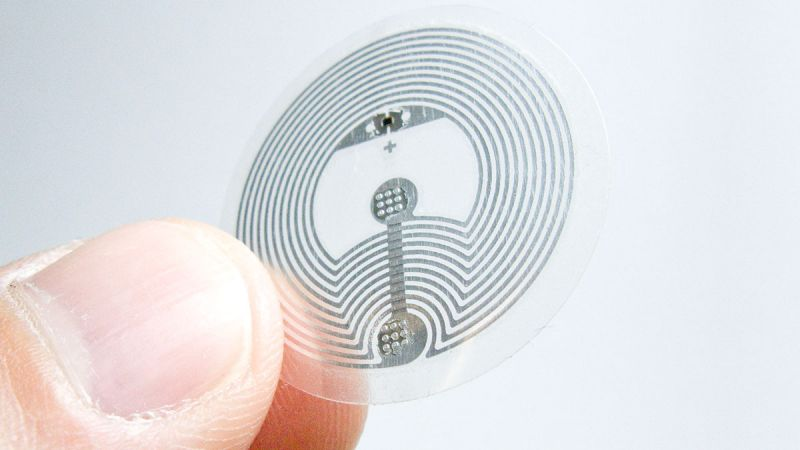
\includegraphics[width=0.25\textwidth]{assets/uitvoering/NFC_chips.jpg}
  \caption{NFC chip}
  \label{fig:uitvoering:NFC_chip}
\end{wrapfigure}
De NFC-feature is een van de killer-features van de NichePlayer. Het is de reden dat een artiest een NichePlayer wil gebruiken. NFC staat voor Near Field Communication, en wordt gebruikt om draadloos informatie uit te wisselen tussen twee apparaten of een apparaat en een kaart. Bekende toepassingen binnen Nederland zijn de OV-chipkaart en contactloos betalen. Binnen de NichePlayer wordt NFC gebruikt om toegang tot de muziek te krijgen. Iedere NFC-chip is uniek, en kan worden gekoppeld aan een album van een NichePlayer Artist. Door een NFC-chip te scannen met een telefoon wordt de toegang gekoppeld met het account van de gebruiker. De gebruiker kan vervolgens de muziek luisteren op alle apparaten die zijn gekoppeld aan het account.

Wanneer een andere telefoon de NFC-chip scant, wordt de chip ook gekoppeld aan het account van die telefoon. Dit kan worden gebruikt om de muziek te delen met vrienden. Er zit echter wel een limiet op het aantal accounts dat gekoppeld kan worden aan een chip. Dit is om te voorkomen dat een gebruiker een chip kan kopen en deze vervolgens kan delen met iedereen. De limiet is in te stellen door de artiest, maar zal standaard ingesteld zijn op 3 gebruikers. Wanneer de limiet is bereikt wordt het account dat als eerste gescand heeft ontkoppeld.

Een groot verschil met bestaande fysieke distributie media is dat de chip slechts een doorgeefluik is. De muziek wordt niet opgeslagen op de chip, maar op de servers van de artiest. Dit betekent dat de muziek altijd up-to-date is, en dat de artiest de muziek kan aanpassen zonder dat de chip opnieuw gemaakt hoeft te worden. Content is daarnaast ook niet gelimiteerd tot muziek, ook andere media zoals video's en foto's zijn mogelijk. De NichePlayer NFC chips zijn daarom een goede vervanger voor de huidige distributie media.

NFC-chips zijn fysieke producten, wat betekend dat er automatisch een beperkte voorraad is. Dit zorgt ervoor dat de chips een hogere waarde hebben dan digitale producten. Er kunnen geen perfecte kopieën van de chips gemaakt worden.

De NFC-chips maken het mogelijk om muziek op een fysieke wijze te verkopen, maar tijdens het afspelen de voordelen van streaming te hebben. De chips zijn makkelijk te verwerken in bestaande producten als Vinyl platen, CD's en andere merchandise, maar bieden meer creativiteit. Daarnaast zijn de chips relatief goedkoop te produceren.

\subsubsection*{NichePlayer Extended Services}
De Extended Services zijn extra functionaliteiten die het gebruik van de NichePlayer Artist verder uitbreiden. De Extended Services zijn optioneel en kunnen per functie worden aangeschaft door de artiest.

Veel van deze functies zijn gebaseerd op technische restricties van de manier waarop de NichePlayer Artist is opgezet. Het gaat hierbij om features die niet via een standaard webserver zoals apache server kunnen lopen, of bepaalde software licenties nodig hebben. Hoewel de extended services in theorie zelf te hosten zijn (via een docker image), vergt dit veel technische kennis. Het is dan ook een goede reden om als ontwikkelaar de extended services apart aan te bieden.

Een van de extended services is een Media Transcoder. Hiermee kan een artiest een enkel hoog kwaliteit bestand uploaden, die vervolgens door het systeem wordt omgezet naar verschillende lagere kwaliteiten. Dit omzetten kost normaal veel tijd, waardoor het voor de artiest nuttig is om uit handen te geven. Dit is een belangrijke functie voor het gebruiksgemak van luisteraars, omdat zij zo zelf kunnen kiezen welke kwaliteit ze willen luisteren. Het versturen van grote bestanden kost veel opslag en bandbreedte, wat op mobiele verbindingen veel geld kost. Als een luisteraar echter thuis is, kan die wel de hoogste kwaliteit luisteren.

De Media Transcoder is een complexe functie die veel CPU-kracht en bepaalde programma's  nodig heeft. Het is daarom niet mogelijk om deze functie op een standaard webserver te draaien. De Media Transcoder wordt daarom aangeboden als een Extended Service.

Een andere extended service is Large File Hosting. Dit staat los van de Hosting Service die hiervoor genoemd is. Deze service is bedoeld voor het hosten van grote bestanden zoals verschillende kwaliteiten van mediabestanden. Door deze bestanden los te halen van de NichePlayer Artist kan de website sneller laden en is het zelf-hosten van de website goedkoper.

\subsubsection*{NichePlayer Hub}
Een van de krachtige features van bestaande streamingdiensten is het vinden van nieuwe muziek en content. Dit is tegenwoordig een van de voornaamste redenen dat artiesten hun muziek publiceren op streamingdiensten.

De NichePlayer Hub is een centrale plek waar luisteraars nieuwe muziek kunnen vinden. De Hub verzamelt de losse NichePlayer Artist websites en bouwt er een algemene streamingdienst omheen. De muziek is nog steeds gehost op de NichePlayer Artist websites, maar de Hub verzameld de muziek en maakt het vindbaar voor luisteraars.

Gebruikers van de Hub vormen vervolgens ook zelf een grote community. \todo{Schrijven over community}

Om zichtbaar te zijn op de Hub moet een artiest een abonnement hebben. Dit abonnement is een vast bedrag per maand. De kosten voor de servers worden gedekt door de maandelijkse betalingen van de artiesten. Daarnaast kan een artiest extra betalen om te hoger in het zoekalgoritme van de Hub te komen. Dit is een extra inkomstenbron voor de NichePlayer.

\subsubsection*{NichePlayer Native Apps}
De NichePlayer is gemaakt als webplatform. Hierdoor is het makkelijk te draaien op verschillende soorten computers, en hoeft er niet voor ieder platform een aparte app te worden gemaakt. Ontwikkeling gaat hierbij snel. Er zijn echter ook nadelen aan deze aanpak. De NichePlayer (en Hub) is niet te vinden in de verschillende appstores waardoor het minder makkelijk te vinden is voor luisteraars. Daarnaast kan een webapp minder goed verbinden met het besturingssysteem van het apparaat, waardoor functies als playback controls van het systeem, offline downloaden van muziek en het afspelen in de auto niet mogelijk zijn.

Voor een native app zou de artiest zelf een ontwikkelaars account moeten hebben om een native app van zijn NichePlayerArtist te kunnen publiceren, wat extra werk is voor de artiest en bovendien veel geld kan kosten afhankelijk van de appstore. Het onderhouden van een app is moeilijker omdat er verschillende versies moeten worden onderhouden voor de verschillende platformen.

Een oplossing is het aanbieden van een overkoepelende NichePlayerApp. Deze app is voornamelijk gericht op de Hub, maar kan ook de NichePlayer Artist websites koppelen en afspelen. Omdat het ontwikkelen van de App veel tijd kost zal deze in eerste instantie alleen de basis functies hebben (i.e. afspelen van muziek). De NichePlayerApp is een native app die beschikbaar is in de verschillende appstores. De app is gratis te downloaden en te gebruiken.

\subsubsection*{NichePlayer Custom development}
Er zijn nog veel meer functionaliteiten te bedenken die de NichePlayer kan bieden. De NichePlayer is een framework, en kan dus worden uitgebreid met nieuwe functionaliteiten. Deze functionaliteiten kunnen worden aangevraagd door middel van offerte bij de ontwikkelaar van de NichePlayer. Hiermee blijft de NichePlayer groeien en kan het worden aangepast aan de wensen van de artiesten.

\subsection {Uitwerken Software}
\subsubsection*{U.F.O.-App}
Ik ben al jaren een framework aan het ontwikkelen waarmee ik snel web-systemen kan opzetten. Dit framework heeft veel verschillende iteraties gezien (begonnen als puur zelf ontwikkeld, nu gebaseerd op verschillende andere libraries). Om de meest recente versie van het framework te testen ben ik de afgelopen 1.5 jaar bezig geweest met het ontwikkelen van een dranksysteem app voor mijn studentenscouting groep de U.F.O.-Stam uit Utrecht. Het concept achter de app heeft verder weinig te maken met de opleiding (verkopen van drankjes en andere producten tijdens de opkomsten). Wat wel relevant is voor de NichePlayer, zijn onderdelen zoals user-authenticatie, media upload en transcodering, User Interface en User Experience design en algehele stabiliteit van het systeem. Met andere woorden, de app is een goede test-case voor het ontwikkelen van de kern van het framework.

Het grote voordeel van het ontwikkelen van deze app voor mijn scoutinggroep is dat ik het framework heb kunnen testen in een realistische live omgeving. Hoewel er in iets meer dan een jaar tijd meer dan 5000 transacties zijn gemaakt met een totale waarde van meer dan €4800,- was het toegestaan om fouten te maken. De app is niet bedoeld voor commerciële doeleinden en de gebruikers zijn bekend met het feit dat het een ontwikkel project is. Dit heeft mij de mogelijkheid gegeven om het framework te testen in een realistische omgeving, zonder dat er grote gevolgen waren als er iets fout ging.

De app is inmiddels stabiel en heeft meer dan 125 gebruikers. Op piekmomenten wordt de app door meer dan 50 mensen tegelijk gebruikt, wat niet mogelijk was met oude versies van het framework tijdens mijn bachelor uitwerking van de NichePlayer.

\subsubsection*{Plugins}
Tijdens de laatste update aan de U.F.O.-App heb ik kern onderdelen van het framework verplaatst naar losse plugins en GIT repositories. Hierbij gaat het onder andere om de API-communicatie, gebruiker authenticatie, media-upload en enkele UI elementen die ik vaak hergebruik. Ik realiseerde mij dat ik deze onderdelen vaak ontwikkel in verschillende projecten, maar iedere keer vanaf scratch begin. Door deze onderdelen te verplaatsen naar losse plugins kan ik ze makkelijk hergebruiken in andere projecten. Dit is ook het geval bij de NichePlayer. De NichePlayer maakt gebruik van verschillende plugins die ik heb ontwikkeld voor de U.F.O.-App. Het grote voordeel van deze plugin-structuur is dat de projecten profiteren van elkaars ontwikkeling. Als ik een update ontwikkel voor de U.F.O.-App, kan ik deze ook vrijwel direct gebruiken in de NichePlayer. Dit zorgt ervoor dat ik sneller kan ontwikkelen en meer kan focussen op de implementatie van de unieke functies van de verschillende systemen, in plaats van de kern van het systeem.

\subsubsection*{API-communicatie}
De NichePlayer maakt gebruik van een API om te communiceren tussen de frontend en de backend. Deze API was in vorige versies van mijn framework gebaseerd op GraphQL. Deze api-vorm gebruikt een enkele endpoint (url) waarnaar een zogenaamde query (een vraag of opdracht) wordt gestuurd. Deze query wordt vervolgens verwerkt door de server en het resultaat wordt teruggestuurd naar de client. Het grote voordeel van GraphQL is dat de client zelf kan bepalen welke data hij nodig heeft. Hierdoor kan de server efficiënter werken en hoeft er minder data over verschillende requests verstuurd te worden. Ingewikkelde en uitgebreide zoekopdrachten zoals "geef mij een album met alle nummers en artiesten, en alle gebruikers die op dit moment naar dit album aan het luisteren zijn" kan in een enkele query verstuurd worden.

GraphQL bleek echter verschillende nadelen te hebben binnen deze uitwerking van het systeem. Zo was het bijvoorbeeld niet mogelijk om queries te cachen en hergebruiken voor verschillende users. Het grootste nadeel was echter een gebrek aan configuratie aan de frontend kant. Ik gebruikte een library die de queries voor mij genereerde, maar deze library bleek niet intelligent of aanpasbaar genoeg. Hierdoor was het niet mogelijk om de queries te optimaliseren voor de verschillende functies van de app. Een voorbeeld was een circulaire referentie die moeilijk op te lossen was. Bij deze circulaire referentie vroeg ik bijvoorbeeld  om een album, waarbij ik automatisch alle tracks van het album mee kreeg. Een track had echter ook een lijst van gebruikers die recent naar dat nummer hadden geluisterd. Deze gebruikers hadden vervolgens weer een lijst van albums die ze hadden gekocht, waarbij ik weer alle tracks van het album kreeg. Dit zorgde ervoor dat de app onnodig veel data moest verwerken en versturen. De cirkel was enkel te doorbreken door het automatisch ophalen van relaties uit te zetten, of handmatig de queries te schrijven in plaats van te laten genereren door de library. Hiermee ging de kracht van het gebruik van de GraphQL library verloren, waardoor het toch makkelijker was om over te stappen naar eenvoudigere API vormen.

De nieuwe API is gebaseerd op REST. Dit is een meer traditionele API-vorm waarbij er verschillende endpoints zijn op de server die verschillende data terugsturen. Het grote voordeel van deze API-vorm is dat het makkelijker is om de data te optimaliseren voor de verschillende functies van de app. Zo kan ik bijvoorbeeld een endpoint maken die enkel de data terugstuurt die nodig is voor het afspelen van een album, en een andere endpoint die voor de administrator van het systeem juist alle data doorstuurt. Dit zorgt ervoor dat de app sneller werkt en minder data hoeft te versturen. De REST-API is meer configuratie werk, maar zorgt voor overzichtelijkere code en een snellere app.

Een voordeel van REST is dat ik de API kan hergebruiken tussen verschillende programmeertalen. De NichePlayer-Artist moet vanwege zijn self-hostable karakter geschreven worden in PHP, terwijl de NichePlayer-Hub geschreven wordt in RubyOnRails. Beide programmeertalen hebben een eigen manier van communiceren met een API, maar door de API te schrijven in een taal-onafhankelijke syntax kan ik de API hergebruiken in beide projecten.

\subsubsection*{NichePlayer-Artist}
Na lang te hebben gewerkt aan de U.F.O.-App was het tijd om de vertaalslag te maken naar de NichePlayer-Artist. Omdat ik in de laatste updates aan de U.F.O.-App had gewerkt met plugins kon ik in erg korte tijd de code strippen en herschrijven. Ik ben uiteindelijk ongeveer 2 dagen bezig geweest met het strippen van de code van het dranksysteem, en vervolgens een dag of 3 met het implementeren van de Minimal Viable Product eisen van de NichePlayer. Dit laatste was voornamelijk mogelijk door het hergebruiken van code van mijn bachelor versie van de NichePlayer en kennis die ik de afgelopen jaren heb opgedaan als developer bij TapTapes.

De NichePlayer-Artist is een simpele muziek player die alleen toegankelijk is met een useraccount. Binnen de player zitten standaard functies zoals het afspelen en pauzeren van muziek, binnen een track seeken, een repeat functie en volume. Daarnaast is er een lijst met alle tracks die worden afgespeeld. De player is responsive en werkt op zowel desktop als mobiel. De achtergrond van de player wordt gegenereerd uit de album cover. De nummers die worden afgespeeld worden opgeslagen in een luistergeschiedenis. Deze geschiedenis wordt naast statistiek en betaling voor de artiest ook gebruikt om de luisteraar te laten zien wat hij heeft geluisterd. Ook kunnen andere luisteraars zien dat een gebruiker naar een bepaald album heeft geluisterd. Dit is een manier om de community te versterken.

De NichePlayer-Artist heeft een administratie paneel die wordt gebruikt om het systeem te beheren. Binnen dit paneel kan de artiest gebruikers beheren, verschillende soorten media beheren en albums toevoegen. Tijdens het uploaden van media analyseert de backend de bestanden en slaat metadata op voor later gebruik. In het geval van audio bestanden wordt de ID3 tag met track info opgeslagen.

\subsubsection*{NichePlayer-Hub}
De NichePlayer-Hub is de centrale plek waar NichePlayer-Artists worden gebundeld tot één systeem. Dit project is opgezet in RubyOnRails. Net als de Artist is de Hub gebaseerd op een bestaand project, die ik heb omgezet door middel van plugins om het ontwikkelen te versnellen.

Wat het ontwikkelen van de Hub complex maakt is de manier waarop de data wordt opgehaald. De Hub moet namelijk de data van alle NichePlayer-Artists ophalen en dit weergeven aan de luisteraar. Moderne browser-restricties zorgen er echter voor dat de Hub alleen beveiligde toegang mag hebben tot NichePlayer-Artists. Dit komt omdat de NichePlayer-Artists op andere domeinen staan, waardoor de Hub er niet zomaar bij mag.

Een oplossing hiervoor is het maken van een speciale user in de NichePlayer-Artist die door de Hub gebruikt kan worden. Deze user heeft speciale rechten, en kan de data ophalen die binnen de Hub nodig zijn. De Hub fungeert hierbij als proxy.

\subsubsection*{NichePlayer-NFC}
Na de koppeling tussen Artist en Hub was het mogelijk om een NFC dienst op te zetten. Deze dienst heeft nog geen toegangscontrole verwerkt, en werkt puur als redirect wanneer een NFC chip wordt gescand.

Iedere NFC chip heeft een unieke code (UID). Deze code kan worden gebruikt om de chip te identificeren. Wanneer de gebruiker de chip scant wordt een URL gegenereerd die bestaat uit een URL op de Hub, de UID van de chip en een counter hoe vaak de chip gescand is (https://hub.nicheplayer.nl/api/nfc/?uid=00000000000000x000000). De Hub herkent vervolgens de UID en zet deze om naar een link van een album op de site van de Artist. De gebruiker wordt vervolgens met een temporary redirect (HTTP307) doorgestuurd naar de site van de Artist.

Hoewel het verplaatsen van de NFC logica naar de Hub al zorgt voor een betere beveiliging, is het nog steeds mogelijk om het URL te kopiëren en te delen met anderen. Een oplossing hiervoor is het meenemen van de scan-counter waardoor het URL maar eenmalig gebruikt kan worden. Er zijn ook NFC-chips die de UID en scan-count versleutelen met een wachtwoord waardoor het niet mogelijk is het URL handmatig aan te passen. Deze chips zijn echter duurder en daarmee niet bruikbaar voor dit prototype.

Een onderdeel dat nog niet is ontwikkeld is het koppelen van accounts aan de NFC-chips. Met deze functie kunnen luisteraars de chip eenmalig scannen en vervolgens overal luisteren. Wanneer een andere luisteraar de chip scant wordt deze ook gekoppeld aan dat account. Dit kan doorgaan tot een bepaald door de artiest in te stellen limiet, waarna de eerste luisteraar wordt ontkoppeld. Een alternatief is het aanbieden van een eenmalige luistermodus waarbij de chip ontkoppeld wordt zodra de sessie is verlopen. Deze twee opties zijn natuurlijk ook te combineren.

% \subsection*{OUTLINE}
% In dit hoofdstuk wordt verslag gegeven van het proces van het onderzoek. Het businessplan zal hier worden uitgewerkt en onderbouwd. Daarnaast zal het ook worden gebruikt om het prototype te kunnen realiseren en testen bij een testpubliek. Dit testen zal worden geprobeerd te doen tijden tijdens het onderzoek, maar dat is afhankelijk van de beschikbare tijd.
